\chapter{Tổng quan về máy tính lượng tử}
\section{Cơ học lượng tử}
Vào những năm đầu của thế kỷ XX, cơ học cổ điển vẫn thống trị với nền tảng là sự phân biệt giữa tính sóng và tính hạt của vật chất, một vật hoặc có tính chất sóng, hoặc có tính chất hạt. Những bằng chứng thực nghiệm tích lũy theo thời gian của một số thí nghiệm đột phá đã chứng minh sự sai lầm trong lý thuyết về lưỡng tính sóng – hạt: thí nghiệm nhiễu xạ của Thomas Young; hiệu ứng quang điện được thực hiện bởi Heinrich Rudolf Hertz. Lý thuyết mới của thế giới hạt vi mô (hạt hạ nguyên tử như electron, photon) mà trong đó có toàn bộ vật chất và ánh sáng biểu thị những hành vi của hạt và sóng.\\
\begin{figure}
    \centering
    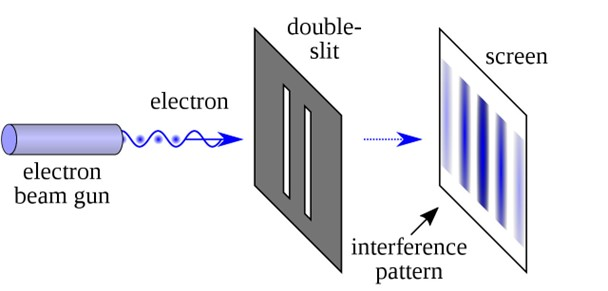
\includegraphics[scale=0.6]{graphics/chapter-1/chapter1-young-experienced.jpg}
    \caption{Thí nghiệm giao thoa ánh sáng của Young}
    \label{fig:my_label}
\end{figure}
\indent Trong thí nghiệm hai khe, ánh sáng chiếu trên màn tối thông qua hai khe hẹp cạnh nhau. Trên màn chắn hứng được những khoảng xen kẽ tối sáng với mức độ khác nhau. Theo lý thuyết vật lý cổ điển, ánh sáng có tính sóng. Những sóng này khi chiếu qua hai khe thì giao thoa với nhau, theo đó mà tăng cường hay triệt tiêu tần số của ánh sáng, dẫn tới xen kẽ sáng tối trên màn chắn.

\indent Cùng cách thức thực hiện, các nhà khoa học chiếu tia proton, electron là các hạt hạ nguyên tử, có tính chất hạt thì nhận được kết quả tương tự. Thí nghiệm đã phủ nhận sự phân biệt giữa sóng và hạt ở cấp độ lượng tử. Nghĩa là, các định luật mà chúng ta sử dụng ở cấp độ nguyên tử từ trước tới nay, có thể không còn đúng ở cấp độ lượng tử.\\
\indent Máy tính hiện đại, càng ngày càng nhỏ gọn với khả năng tính toán lớn. Khả năng xử lý của chúng dựa vào các chip xử lý, mà nói đến tận cùng là các cổng bán dẫn. Từ lúc máy tính đầu tiên được chế tạo, kích thước các bóng bán dẫn đã được nghiên cứu và giảm xuống kích thước chỉ còn vài nanomet, cận kề kích thước nguyên tử. Để tiếp tục tăng khả năng tính toán, ý tưởng về việc chế tạo các cổng bán dẫn với kích thước hạ nguyên tử được đề xuất. Tuy vậy, như thí nghiệm trên, các hạt hạ nguyên tử có những tính chất khác cơ học cổ điển, trong khi máy tính hiện đại vốn được xây dựng trên vật lý cổ điển, vì vậy khả năng tạo ra một máy tính hiện đại với các bóng bán dẫn có kích thước lượng tử là không khả thi. Đây chính là động lực nghiên cứu máy tính lượng tử, dựa trên nền tảng của cơ học lượng tử.
\section{Lược sử các nghiên cứu về máy tính lượng tử}
Năm 1982, nhà vật lý đoạt giải Nobel Laureate Richard Feynman trao đổi rằng máy tính truyền thống không thể mô phỏng toàn bộ tự nhiên. Vật lý truyền thống mô tả tự nhiên một cách chính xác, cố định, xác định và chắc chắn. Tuy nhiên, thực tế tự nhiên thì không phải như vậy, cơ học lượng tử đã chứng minh được điều đó. Vì vậy, cần xuất hiện một loại máy tính mới có khả năng mô tả được cơ học lượng tử \cite{feynman2018simulating}. Năm 1985, David Deutsch của Oxford University đề xuất một máy tính Turing lượng tử và chỉ ra được một thuật toán được thiết kế để chạy trên máy tính lượng tử \cite{deutsch1985quantum}. Năm 1994, Peter Shor đề xuất một thuật toán chạy trên máy tính lượng tử, với khả năng phân tích các số lớn thành tích của hai số nguyên tố với tốc độ nhanh hơn cấp số nhân so với máy tính truyền thống \cite{shor1994algorithms}. \\
\indent
So với các hướng nghiên cứu trong ngành khoa học máy tính nói chung, máy tính lượng tử có lịch sử khá non trẻ. Tuy vậy, những nghiên cứu về nó cũng không kém nhiều so với các ngành khác. Các nghiên cứu về máy tính lượng tử và các lĩnh vực liên quan tăng trưởng ổn định qua các năm, thực sự bắt đầu vào năm 1994 và gia tăng mạnh kể từ năm 2015, lên tới hơn 48,000 ấn phẩm. Các ấn phẩm này chủ yếu là các bài báo. Tính mới và sự phát triển nhanh chóng của lĩnh vực này được phản ánh trong tỷ lệ cao các ấn phẩm xuất hiện từ các hội nghị (21\%), cao gấp đôi so với tỷ lệ chung của các bài báo hội nghị trong Scopus (11\%)\cite{elsevie2021quantum}.
\begin{figure}
    \centering
    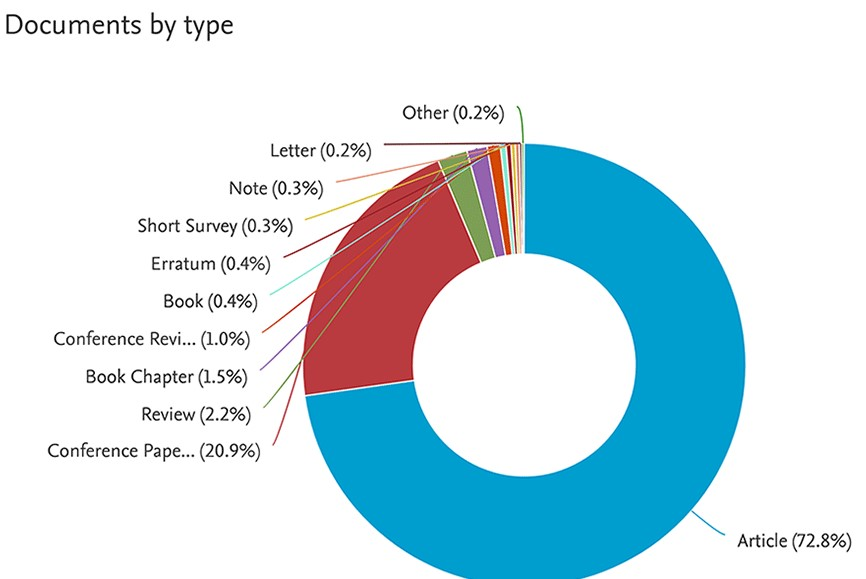
\includegraphics[scale=0.5]{graphics/chapter-1/chapter1-document-by-type.jpg}
    \caption{Phân loại ấn phẩm nghiên cứu về quantum computing từ 1982-2020 \cite{elsevie2021quantum}}
    \label{fig:my_label}
\end{figure} \\
\indent Mười tổ chức có số lượng xuất bản cao nhất nằm ở Trung Quốc, Pháp, Canada, Hoa Kỳ, Vương quốc Anh và Singapore. Viện Hàn lâm Khoa học Trung Quốc cho thấy số xuất bản đặc biệt cao. Tổng chi tiêu của Trung Quốc cho các công nghệ lượng tử, bao gồm cả máy tính lượng tử không được công bố. Tuy nhiên, sự quan tâm của chính phủ đối với việc tài trợ cho các công nghệ lượng tử là rõ ràng trong kế hoạch 5 năm 2016 – 2020 \cite{Quantique2018quantum} và 2021 – 2025 \cite{cuckhoahoc2021quantum} và khoản đầu tư 10 tỷ USD để xây dựng cơ sở nghiên cứu lượng tử lớn nhất thế giới \cite{jeffrey2017quantum}.

\section{Lợi thế của máy tính lượng tử}
\indent Khả năng quan trọng nhất của máy tính lượng tử là tính toán song song, nó có thể xử lý tới 2,5 Extrabyte hàng ngày. Máy tính lượng tử có thể giải quyết những vấn đề toán học phức tạp mà máy tính truyền thống không thể giải quyết được trong thời gian thực tế (phá các thuật toán mã hóa).\\
\indent Hiện tượng “quantum tunneling” làm máy tính lượng tử có thể hoạt động song song và giảm tiêu thụ điện năng từ 100 – 1000 lần. Từ đó, nhiệt lượng tỏa ra cũng giảm đáng kể.\\
\indent Nhìn chung, máy tính lượng tử nhanh hơn hàng nghìn lần so với máy tính cổ điển. Nó dễ dàng giải quyết các vấn đề phức tạp trong tính toán như tìm tuyến đường tốt nhất và lên lịch các chuyến tàu và chuyến bay. Nó cũng có thể tính toán 1 nghìn tỷ nước đi trong cờ vua mỗi giây. Máy tính lượng tử sẽ có thể bẻ khóa các kỹ thuật mã hóa tốt nhất. Tuy nhiên, nó cũng sẽ xây dựng các giải pháp thay thế chống hack. Việc phát minh ra các loại thuốc mới sẽ trở nên khả thi. Các thuật toán thị trường của các tổ chức tài chính có thể được cải thiện. Ứng dụng máy tính lượng tử trong trí tuệ nhân tạo sẽ sớm được thử nghiệm \cite{marella2020introduction}.


\section{Một số điểm còn hạn chế}
\begin{itemize}
    \item Máy tính lượng tử, hoàn toàn khác so với máy tính truyền thống. Vì vậy, một số công việc ít đòi hỏi xử lý dữ liệu hay tính toán lớn, máy tính truyền thống có hiệu suất cao hơn.
    \item Máy tính lượng tử vẫn chưa được phát triển hoàn chỉnh. Các tổ chức, chính phủ mới chỉ đang nghiên cứu, những quy chuẩn chung về máy tính lượng tử vẫn chưa được hình thành.
    \item Bởi vận hành phi truyền thống, dựa trên các hạt hạ nguyên tử, nên chúng rất dễ hư hỏng. Sự suy biến của lượng tử, bản chất xác suất của nó là thách thức khi kết quả nó tính ra đôi khi cũng mang tính xác suất.
    \item Sản xuất và vận hành bộ xử lý của máy tính lượng tử rất khó khăn, nó hoạt động không ổn định và khó kiểm tra. Điều kiện để duy trì sự ổn định của nó ở mức 0,2 độ K, thấp hơn nhiệt độ vũ trụ. Rất khó để duy trì và điều chỉnh nhiệt độ như vậy. Làm sao để thương mại hóa chính cổ máy này là câu hỏi chưa có lời giải.
    \item Ngoài những hạn chế về mặt kỹ thuật, hạn chế về mặt xã hội như người xấu có thể lợi dụng khả năng tính toán mạnh của máy tính lượng tử để phạm tội. Những điều như vậy tuy không được đề cập tới nhưng là có tồn tại trong thực tế.
\end{itemize}
